% Construction : racine en (0, 0) ; les quatre groupes en x = 2,6, aux ordonnées
% 2,7 / 0,9 / −0,9 / −2,7 ; les deux rhésus en x = 5,4, décalés de ±0,55.
% La branche cherchée porte un point d'interrogation : c'est la question.
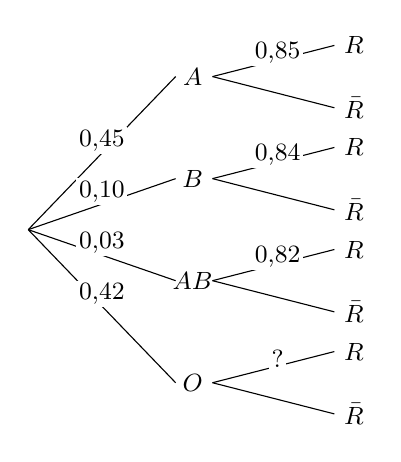
\begin{tikzpicture}[scale=0.72, font=\small]
  \coordinate (R) at (0, 0);
  \foreach \y/\g/\p in {2.7/A/0{,}45, 0.9/B/0{,}10, -0.9/AB/0{,}03, -2.7/O/0{,}42} {
    \draw (R) -- (2.6, \y);
    \node at (2.9, \y) {$\g$};
    \node[fill=white, inner sep=1pt] at (1.3, {\y / 2 + 0.22}) {$\p$};
  }
  \foreach \y/\p in {2.7/0{,}85, 0.9/0{,}84, -0.9/0{,}82} {
    \draw (3.25, \y) -- (5.4, {\y + 0.55});
    \draw (3.25, \y) -- (5.4, {\y - 0.55});
    \node[right] at (5.4, {\y + 0.55}) {$R$};
    \node[right] at (5.4, {\y - 0.55}) {$\bar{R}$};
    \node[fill=white, inner sep=1pt] at (4.4, {\y + 0.42}) {$\p$};
  }
  \draw (3.25, -2.7) -- (5.4, -2.15);
  \draw (3.25, -2.7) -- (5.4, -3.25);
  \node[right] at (5.4, -2.15) {$R$};
  \node[right] at (5.4, -3.25) {$\bar{R}$};
  \node[fill=white, inner sep=1pt] at (4.4, -2.28) {$?$};
\end{tikzpicture}
